%% F3
\begin{figure*}[ht]
  \begin{subfigure}{.4\textwidth}
    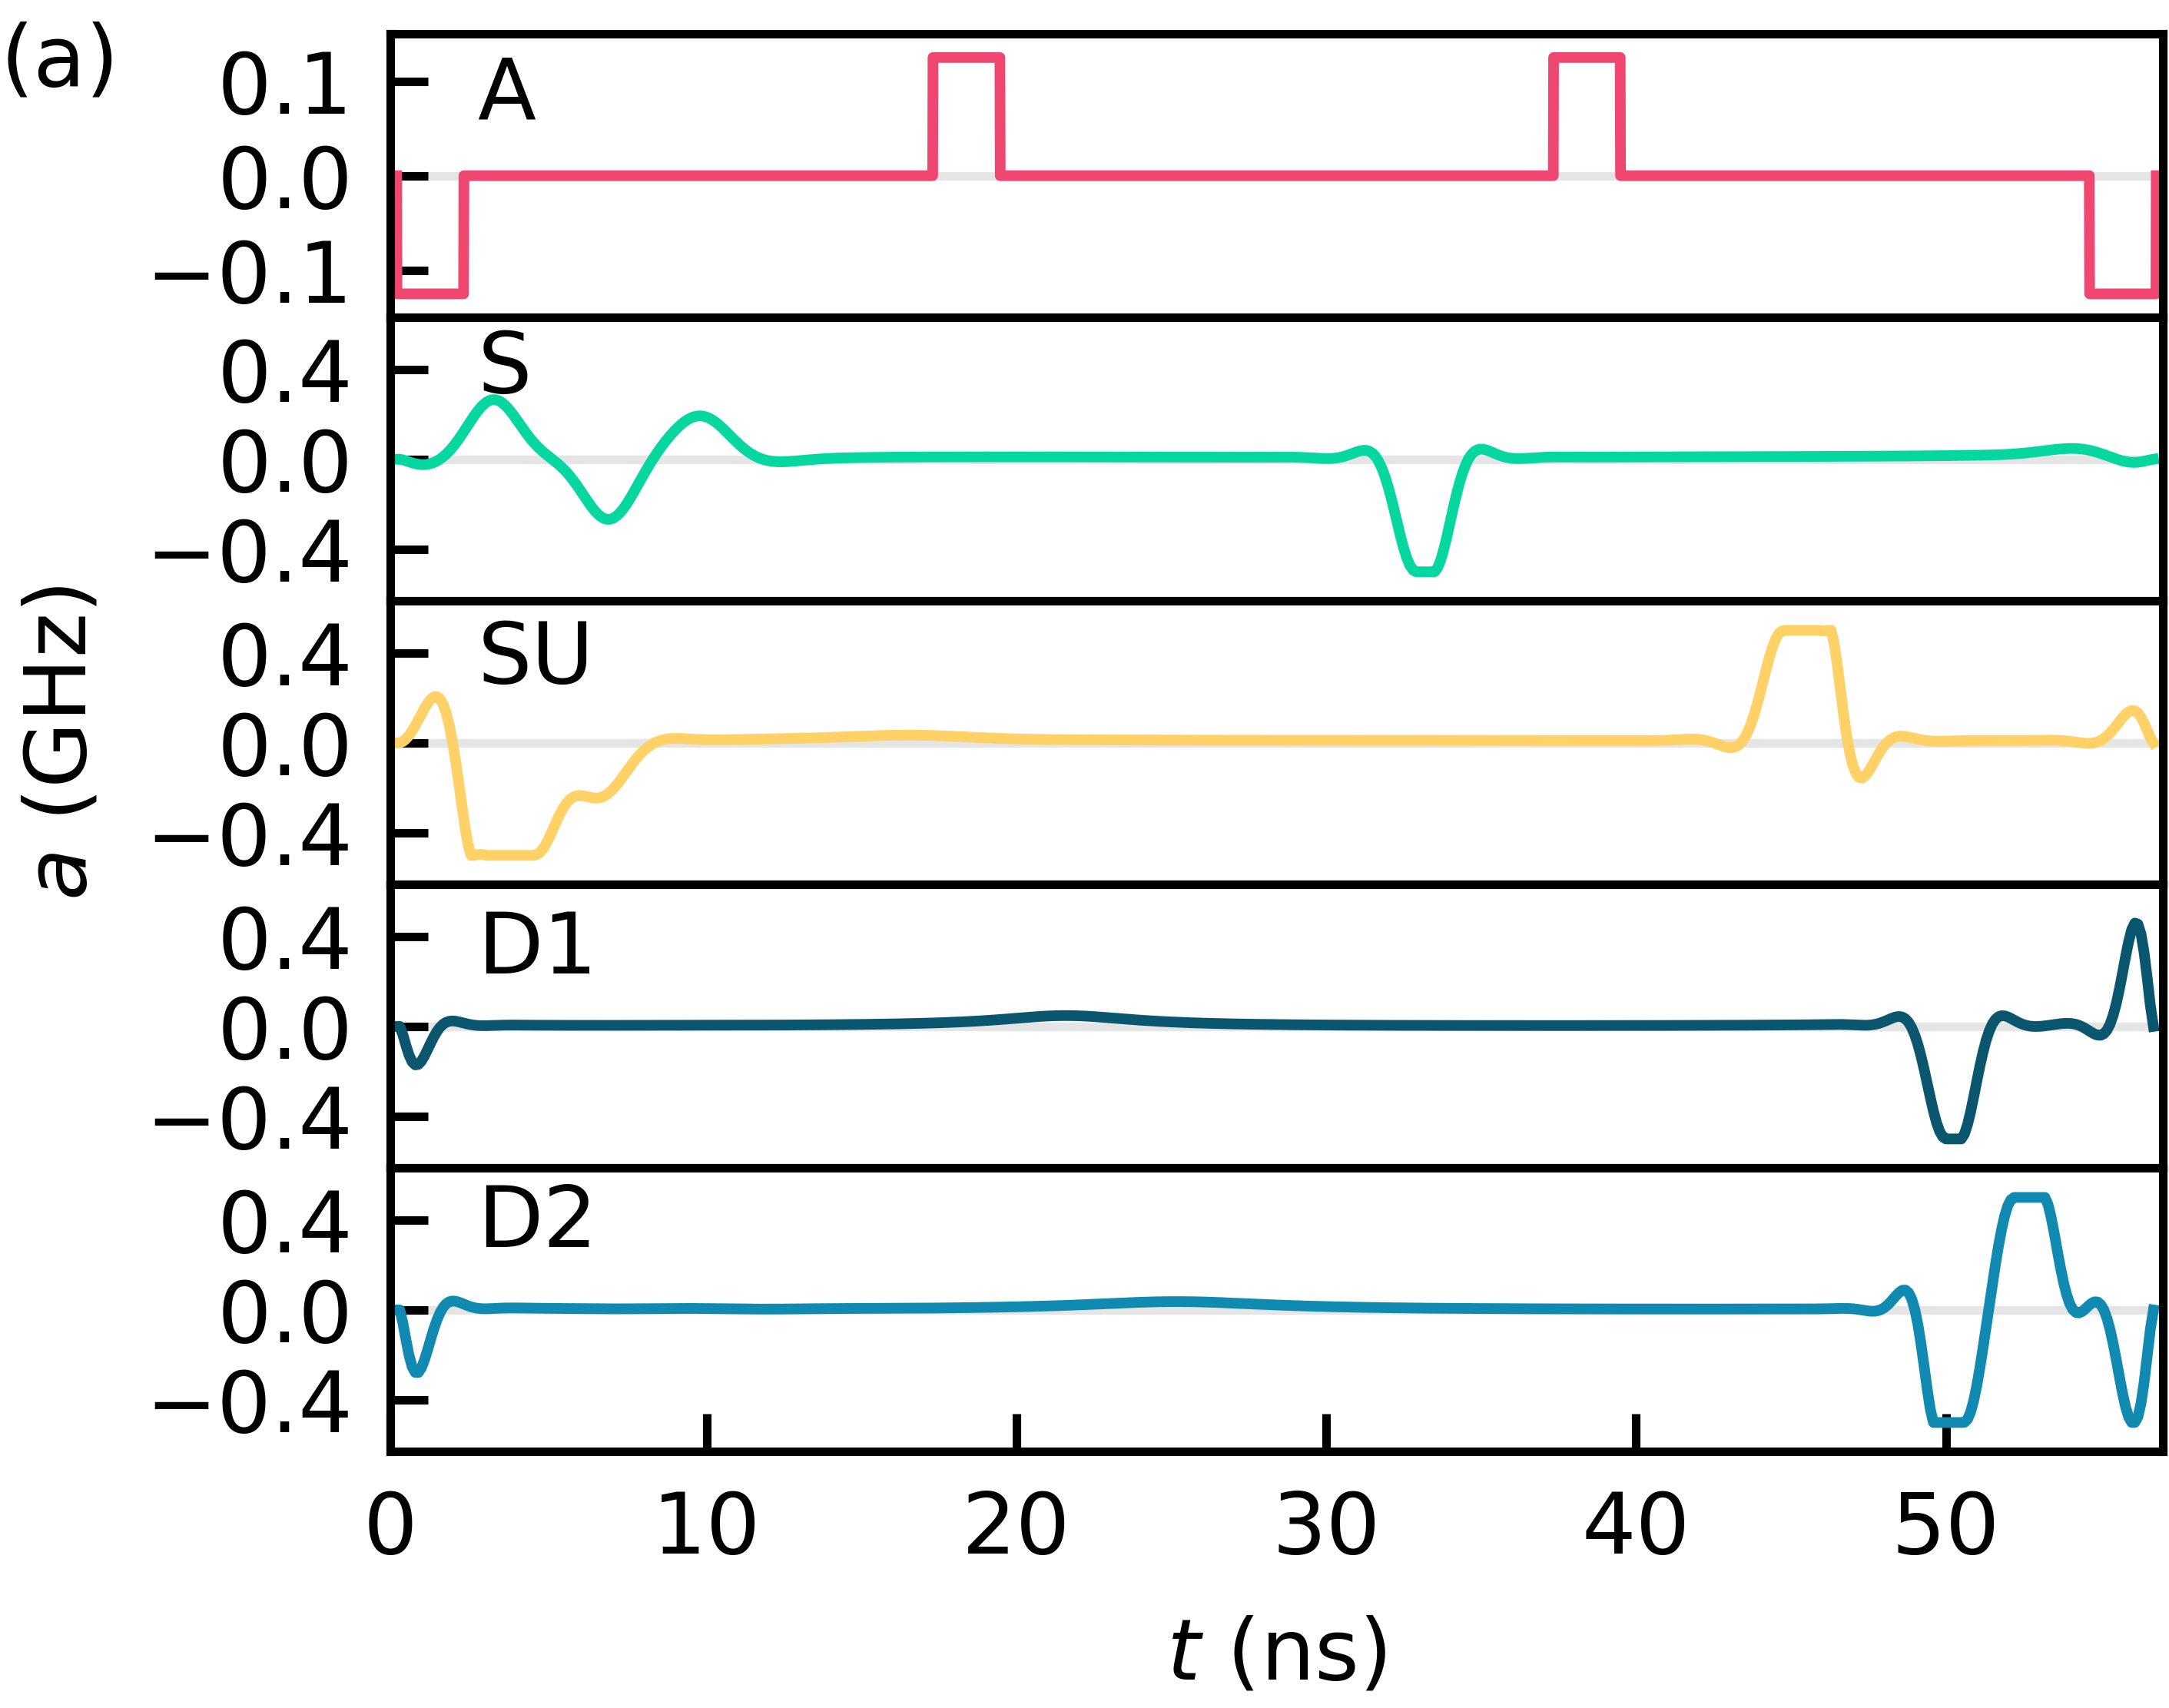
\includegraphics[width=\linewidth]{assets/f3a.png}
    \caption{}
    \label{fig:stochastica}
  \end{subfigure}\hspace{0.05\textwidth}
  \begin{subfigure}{.4\textwidth}
    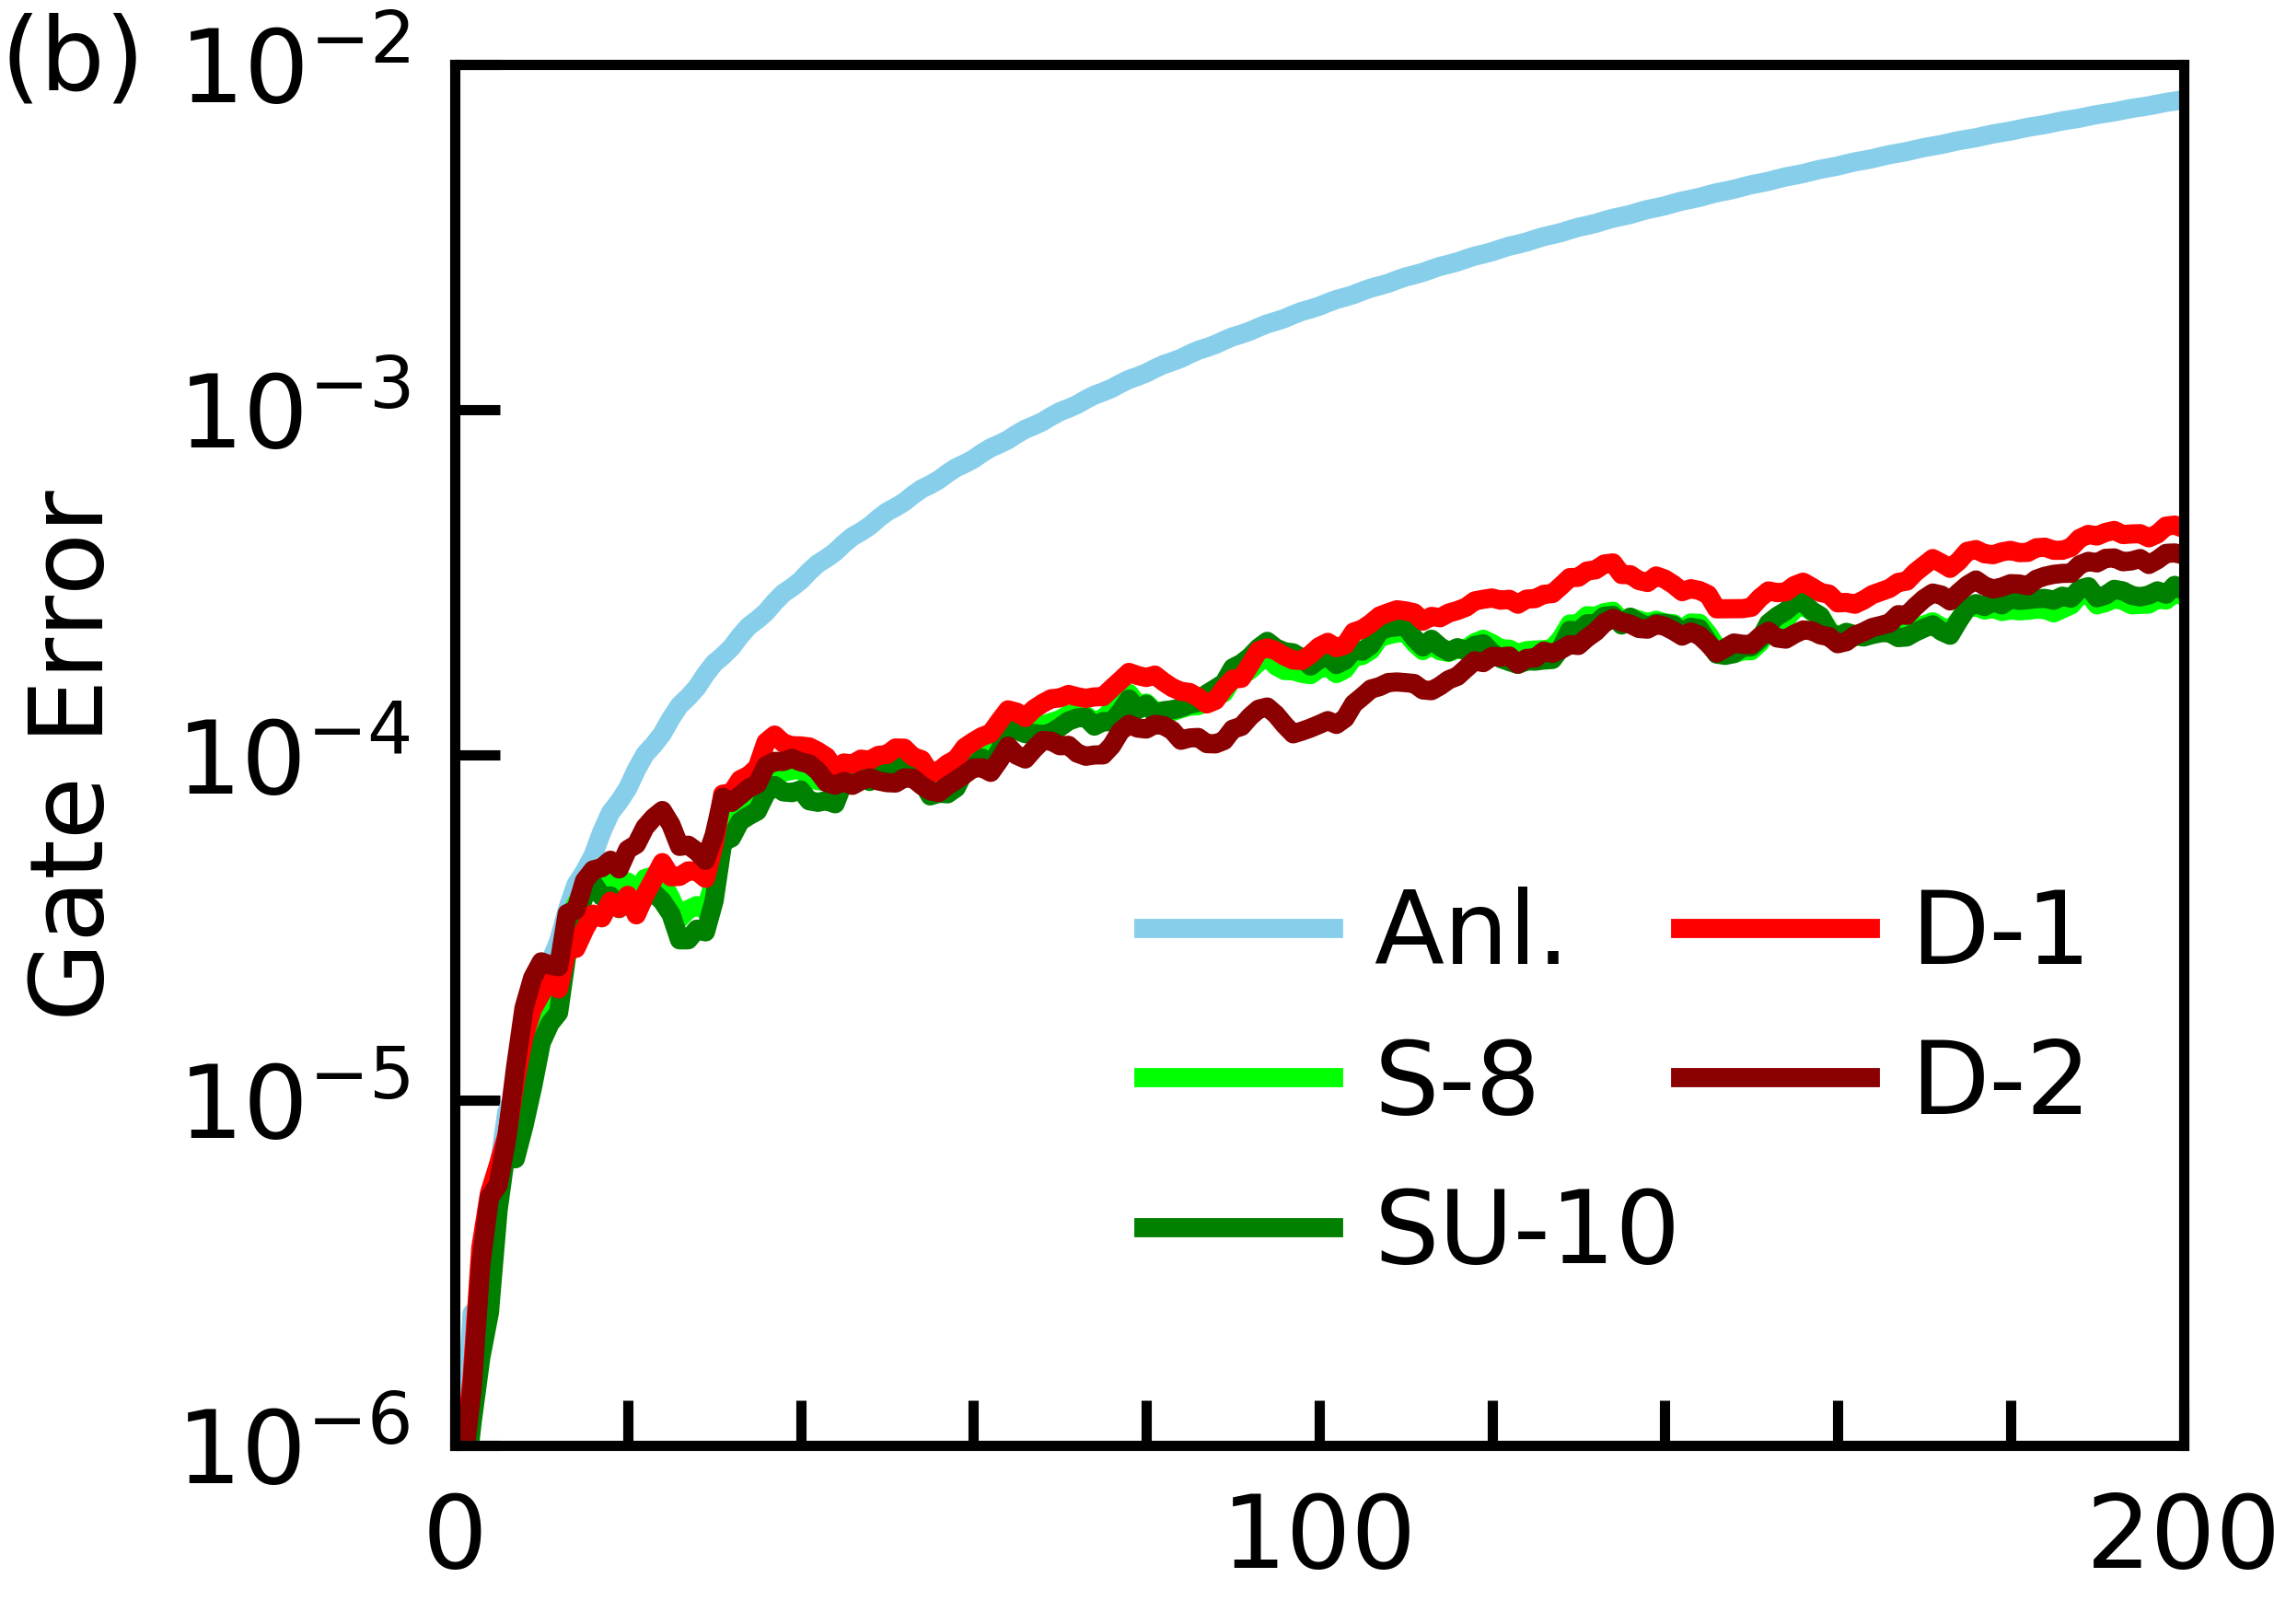
\includegraphics[width=\linewidth]{assets/f3b.png}
        \caption{}
    \label{fig:stochasticb}
  \end{subfigure}
  \caption{
    (a) Flux pulses for $X/2$ gates robust to flux noise
    constructed with the analytic (A),
    sampling (S), unscented sampling (U), and the 1\textsuperscript{st}-
    and 2\textsuperscript{nd}-order derivative methods (D1, D2).
    (b) Cumulative gate error due to 1/$f$ flux noise for
    successive gate applications. The cumulative gate errors for the
    sampling, unscented sampling, and the derivative methods are indistinguishable.
  }
  \label{fig:stochastic}
\end{figure*}

\section{Robustness to Time-Dependent Parameter Uncertainty \label{sec:stochastic}}
An additional source of experimental error arises from time-dependent
parameter uncertainty. For many flux-biased and inductively-coupled
superconducting circuit elements, magnetic flux noise is the dominant
source of coherent errors \cite{bialczak20071f, kakuyanagi2007dephasing,
  kumar2016origin, yoshihara2006decoherence}. Flux noise
modifies the fluxonium Hamiltonian \eqref{eq:hamiltonian}
by $a(t) \rightarrow a(t) + \delta a(t)$ where $\delta a(t)$ is the flux noise.
The spectral density of flux noise is observed to
follow a 1/$f$ distribution
\cite{bialczak20071f, koch2007model, kakuyanagi2007dephasing,
  kumar2016origin, yoshihara2006decoherence, yoshihara2010correlated,
  zhang2020universal},
so the noise is dominated by low-frequency components.
The analytic gate considered here
takes advantage of the low-frequency characteristic and
treats the noise as quasi-static, performing a generalization of the spin-echo
technique to compensate for erroneous drift \cite{hahn1952spin, meiboom1958modified}.

We modify the robust control techniques presented
in the previous section to combat 1/$f$ flux noise.
The unscented sampling method is modified so that the sample states
are subject to 1/$f$ flux noise. The noise
is generated by filtering white noise sampled from a standard
normal distribution with a finite impulse response filter \cite{saspweb2011}.
The noise is then scaled by the 
flux noise amplitude of our device $A_{\Phi} = 5.21 \mu \Phi_{0} \implies
\sigma_{a} = 2.5 \cdot 10^{-5} \textrm{GHz}$.
In principle, we could modify the sampling method
similarly; however, we choose to subject the sample states
to static noise
$a(t) \rightarrow a(t) \pm \sigma_{a}$
for comparison. The derivative methods require no algorithmic modification
from the static case, but the TDSE is now differentiated with respect
to $a(t)$ instead of $f_{q}$ as in \eqref{eq:d1dyn}.

We analyze the gate errors due to 1/$f$ flux noise for
the $X/2$ gates constructed with the robust control techniques
and the analytic $X/2$ gate. To compute the gate error,
we evolve an initial state
under the fluxonium Hamiltonian \eqref{eq:hamiltonian}
where the optimized flux is modified $a(t) \rightarrow a(t) + \delta a(t)$.
We generate the flux noise as
we described for the unscented sampling method.
The reported gate error is the infidelity
averaged over $1000$ pseudorandomly generated initial states,
each of which is subject to a distinct pseudorandomly
generated flux noise instance.
To observe the effect of interfering coherent errors,
we simulate successive applications of the gate constructed by each method;
we compute the cumulative gate error
after each application, see Fig. \ref{fig:stochastic}.
Both the analytic
and numerical gates yield single-gate errors
sufficient for quantum error correction.
Despite converging on qualitatively different solutions, the
numerical gates perform similarly in the concatenated
gate application comparison. Their gate errors
after $200$ gate applications $\sim 11 \mu\textrm{s}$ are
two orders of magnitude less than the gate error produced by the analytic gate.
1/$f$ flux noise is a significant source of coherent errors in NISQ applications,
and these numerical techniques offer effective avenues to mitigate it.
